\subsection{Introduction}
	This section is divided in two parts, the first one describe the implementation of the algorithm in a laptop computer. The objective is to get a reference to compare the results of the final implementation. The second one is a description of the final application and its results.

\subsection{Complete Test in PC}
	In this situation, the algorithm runs in a Desktop computer using a USB camera. Summarizing:
	
	\begin{itemize}
		\item{Camera: 30 Hz and pictures of 640x480}
		\item{Intel core i7 2.20 GHz. Usage 7\%}
		\item{6 GB of RAM. Usage $\sim$ 5000 KB}
	\end{itemize}
	
	\begin{figure}[h]
		\centering
		\begin{subfigure}{0.49\linewidth}
			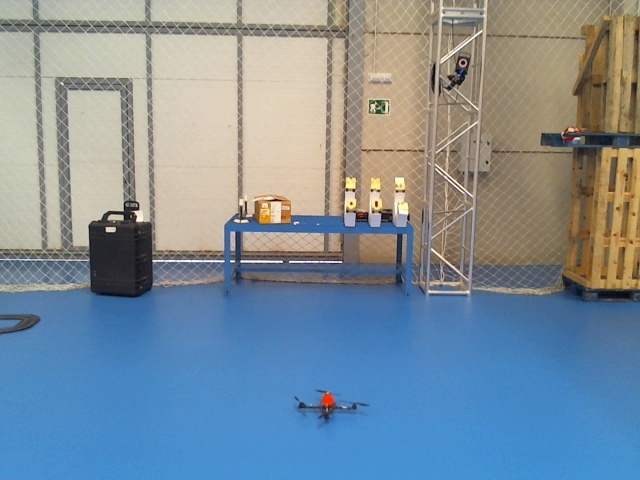
\includegraphics[width=\linewidth]{../Images/c4/image_ori}
			\caption{Original Image}
			\label{fig:image_ori}
		\end{subfigure}
		%--------------------------------------------------------------------
		\begin{subfigure}{0.49\linewidth}
			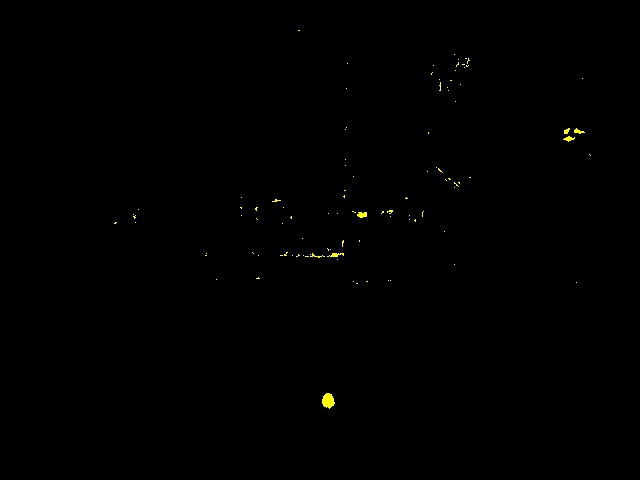
\includegraphics[width=\linewidth]{../Images/c4/image_seg}
			\caption{Segmented Image}
			\label{fig:image_seg}
		\end{subfigure}
	\end{figure}
	
	\begin{figure}[ht]
		\centering
		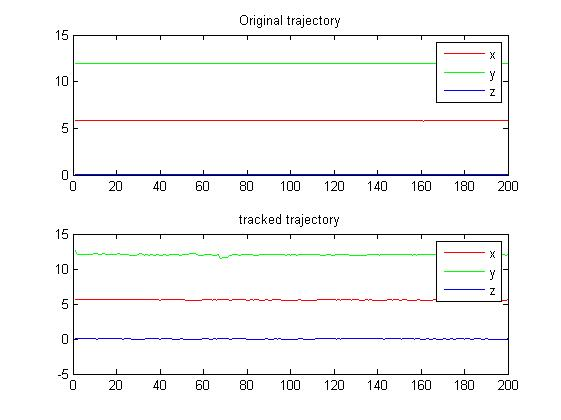
\includegraphics[width=\linewidth]{../Images/c4/trajs}
		\caption{}
		\label{fig:trajectories_PC}
	\end{figure}
	
	\begin{figure}[ht]
		\centering
		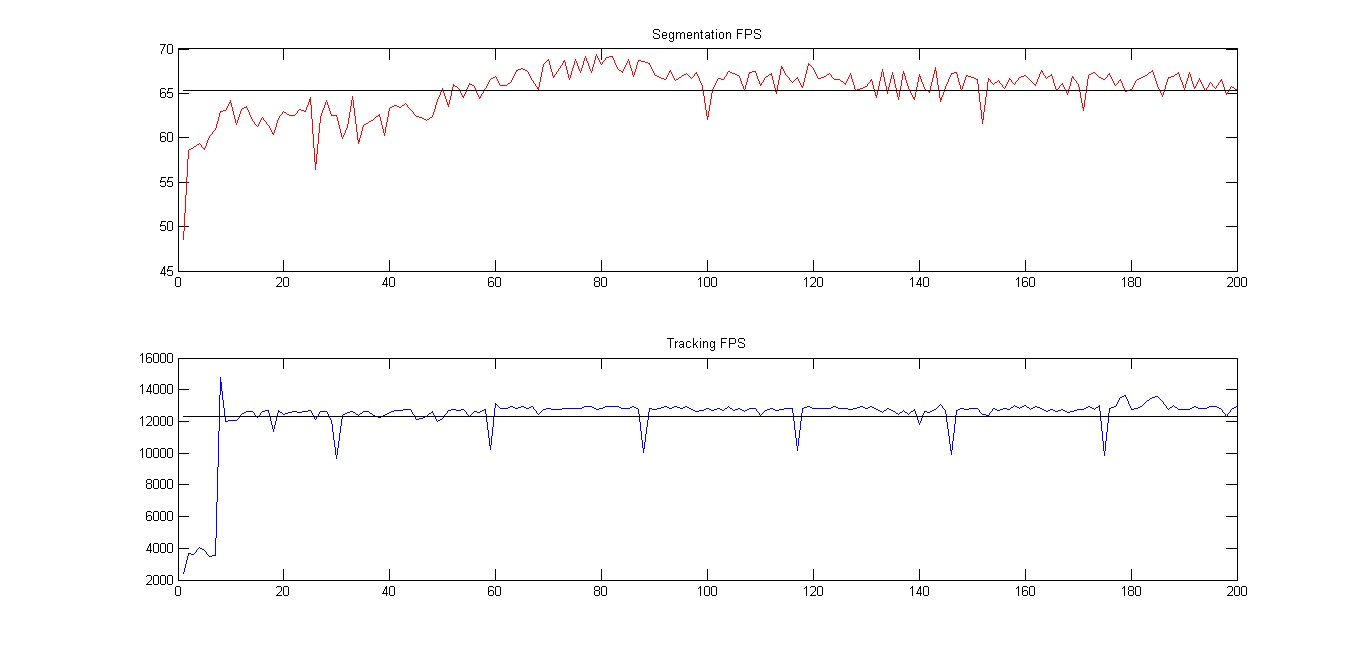
\includegraphics[width=\linewidth]{../Images/c4/fps}
		\caption{}
		\label{fig:fps_PC}
	\end{figure}
		

	

	
\subsection{Test with Odroid and Ground Station}